These sensitivity studies are used to analyze the effects of the parameters that represent \gls{MSR} physical phenomena. 
Polynomial fits of group parameters.
Using \gls{MSRE} temperature and salt density \cite{robertson1965msre}.
No reprocessing unless specified.


\begin{table}[H]
    \centering
    \begin{tabular}{lll}
        \hline
       Parameter  & Value & Units \\
       \hline
        OpenMC Batches & 10 & - \\
        OpenMC Particles & 50000 & - \\
        OpenMC Depletion Chain & ENDF/B-VIII.0 & - \\
        OpenMC Cross Sections & ENDF/B-VIII.0 & - \\
        OpenMC Source Particles & $4.2\times 10^{16}$ & -\\
        Temperature & 920 & $K$\\
        Neutron Energy & $0.0253$ & $eV$\\
        Sample Nuclide & $^{235}U$ & -\\
        Sample Density & 2.3275 & $\frac{g}{cm^3}$\\
        In-core Residence Time & 600 & $s$\\
        Ex-core Residence Time & - & $s$\\
        Irradiation Time & 600 & $s$\\
        Decay Time & 600 & $s$\\
        Decay Time Step & 1 & $s$\\
        \hline
    \end{tabular}
    \caption{Default parameters used for study on \gls{MSR} phenomena in 0D flow \gls{DNP} group parameter formulation OpenMC simulations.}
    \label{tab:params-msr}
\end{table}

\subsubsection{Removal Rates}
\label{sec:repr-scale}

\subsubsection{In and Ex-core Residence Times}
\label{sec:res-time-var}
Compare with static.
\gls{MSRE} is approximately 10 seconds in-core and 15 seconds ex-core \cite{robertson1965msre}.

\begin{figure}[H]
    \centering
    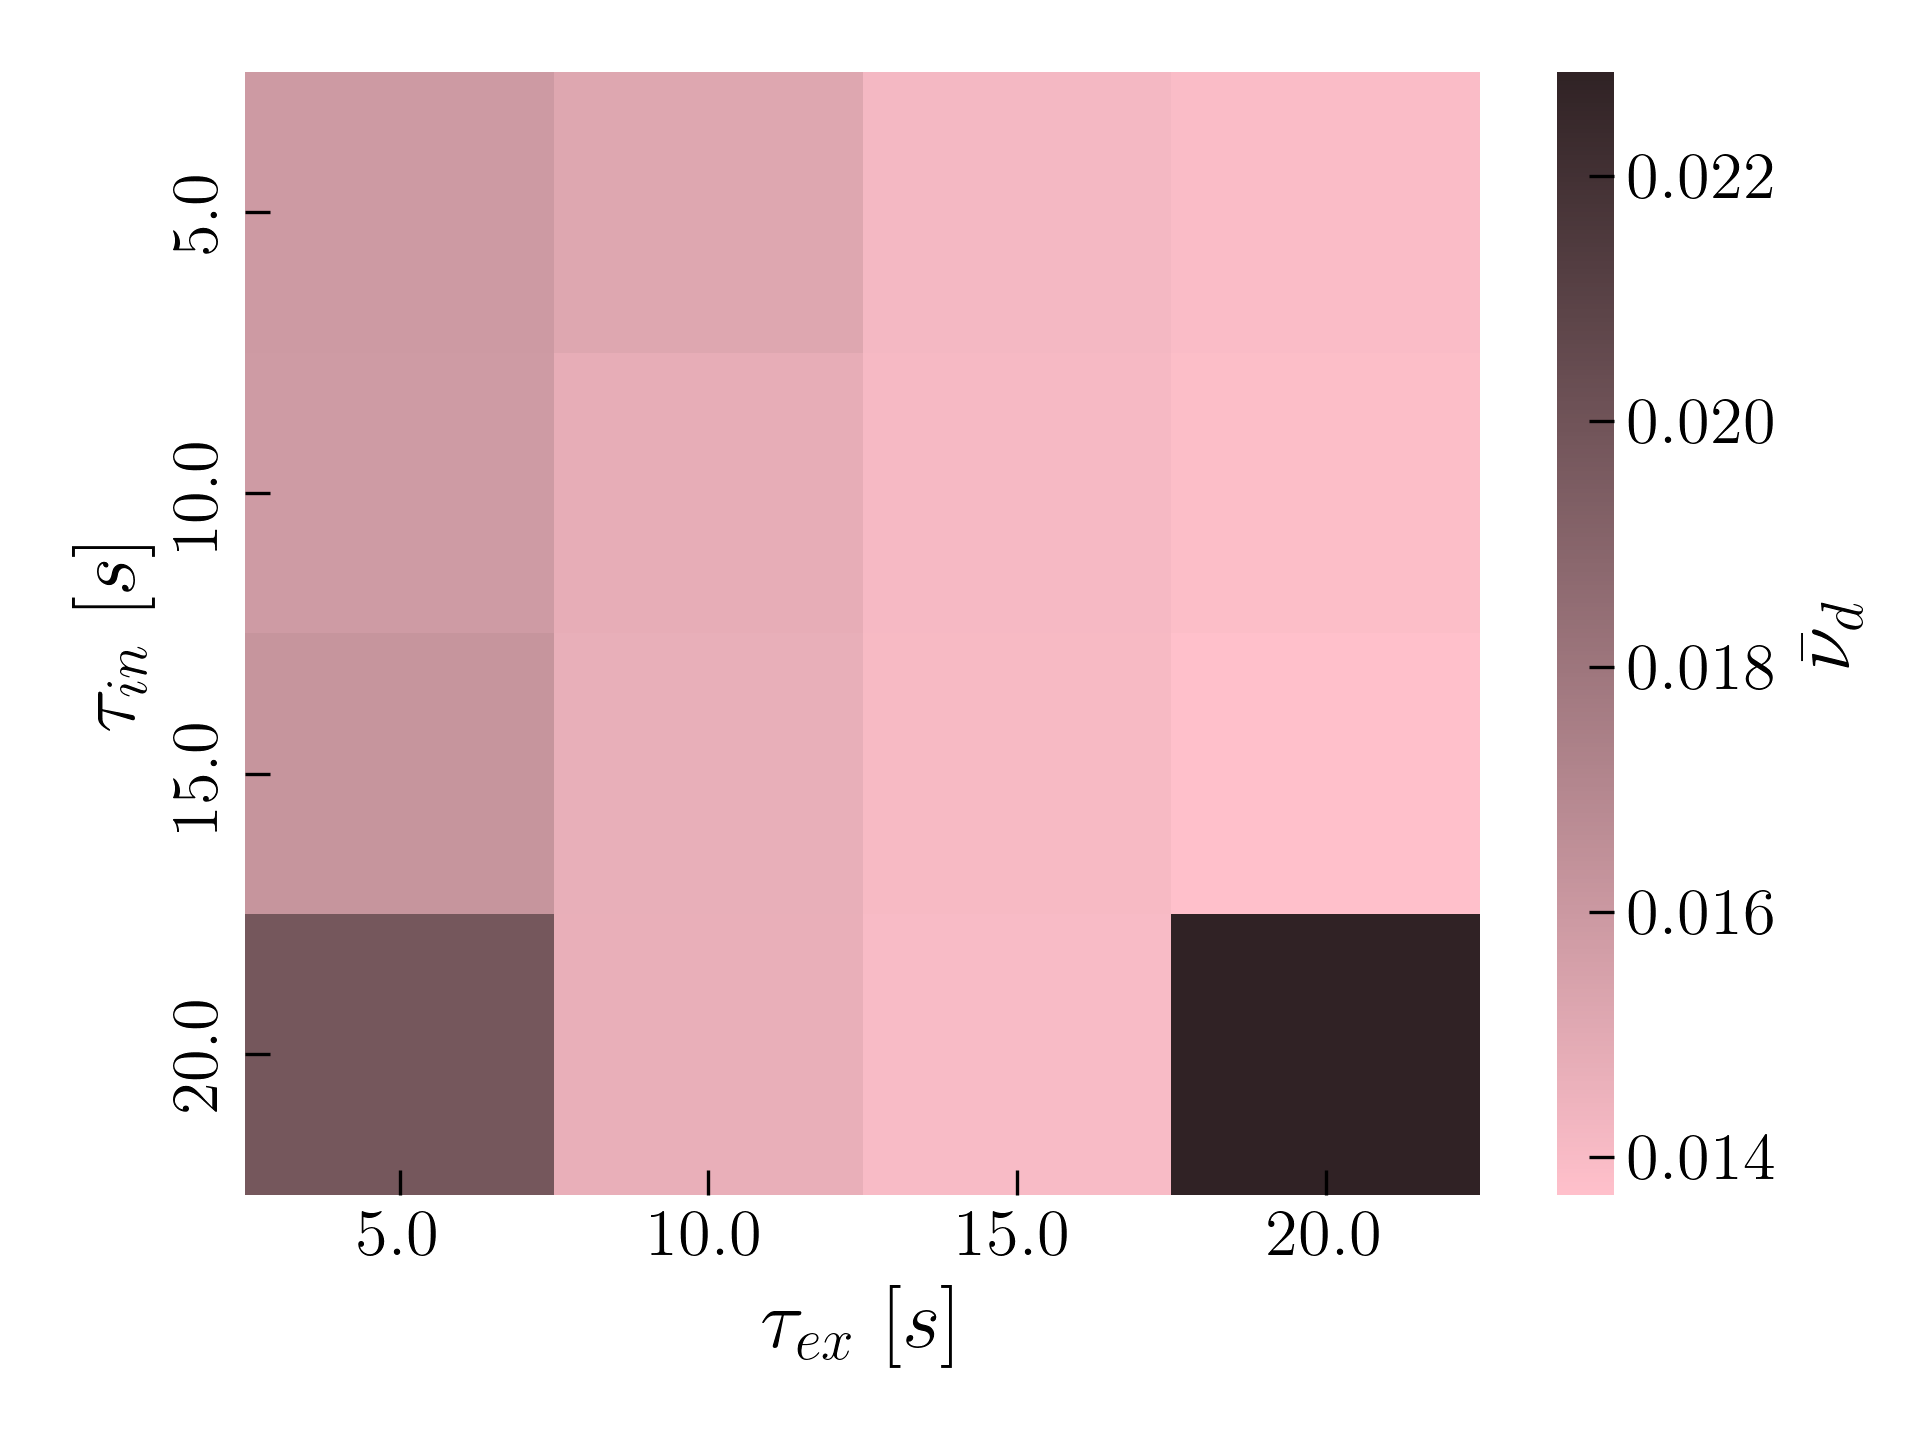
\includegraphics[width=\linewidth]{images/surf-times.png}
    \caption{Total delayed neutron yield for various residence times during irradiation in OpenMC.}
    \label{fig:totyields-restimestudy}
\end{figure}

\begin{figure}[H]
    \centering
    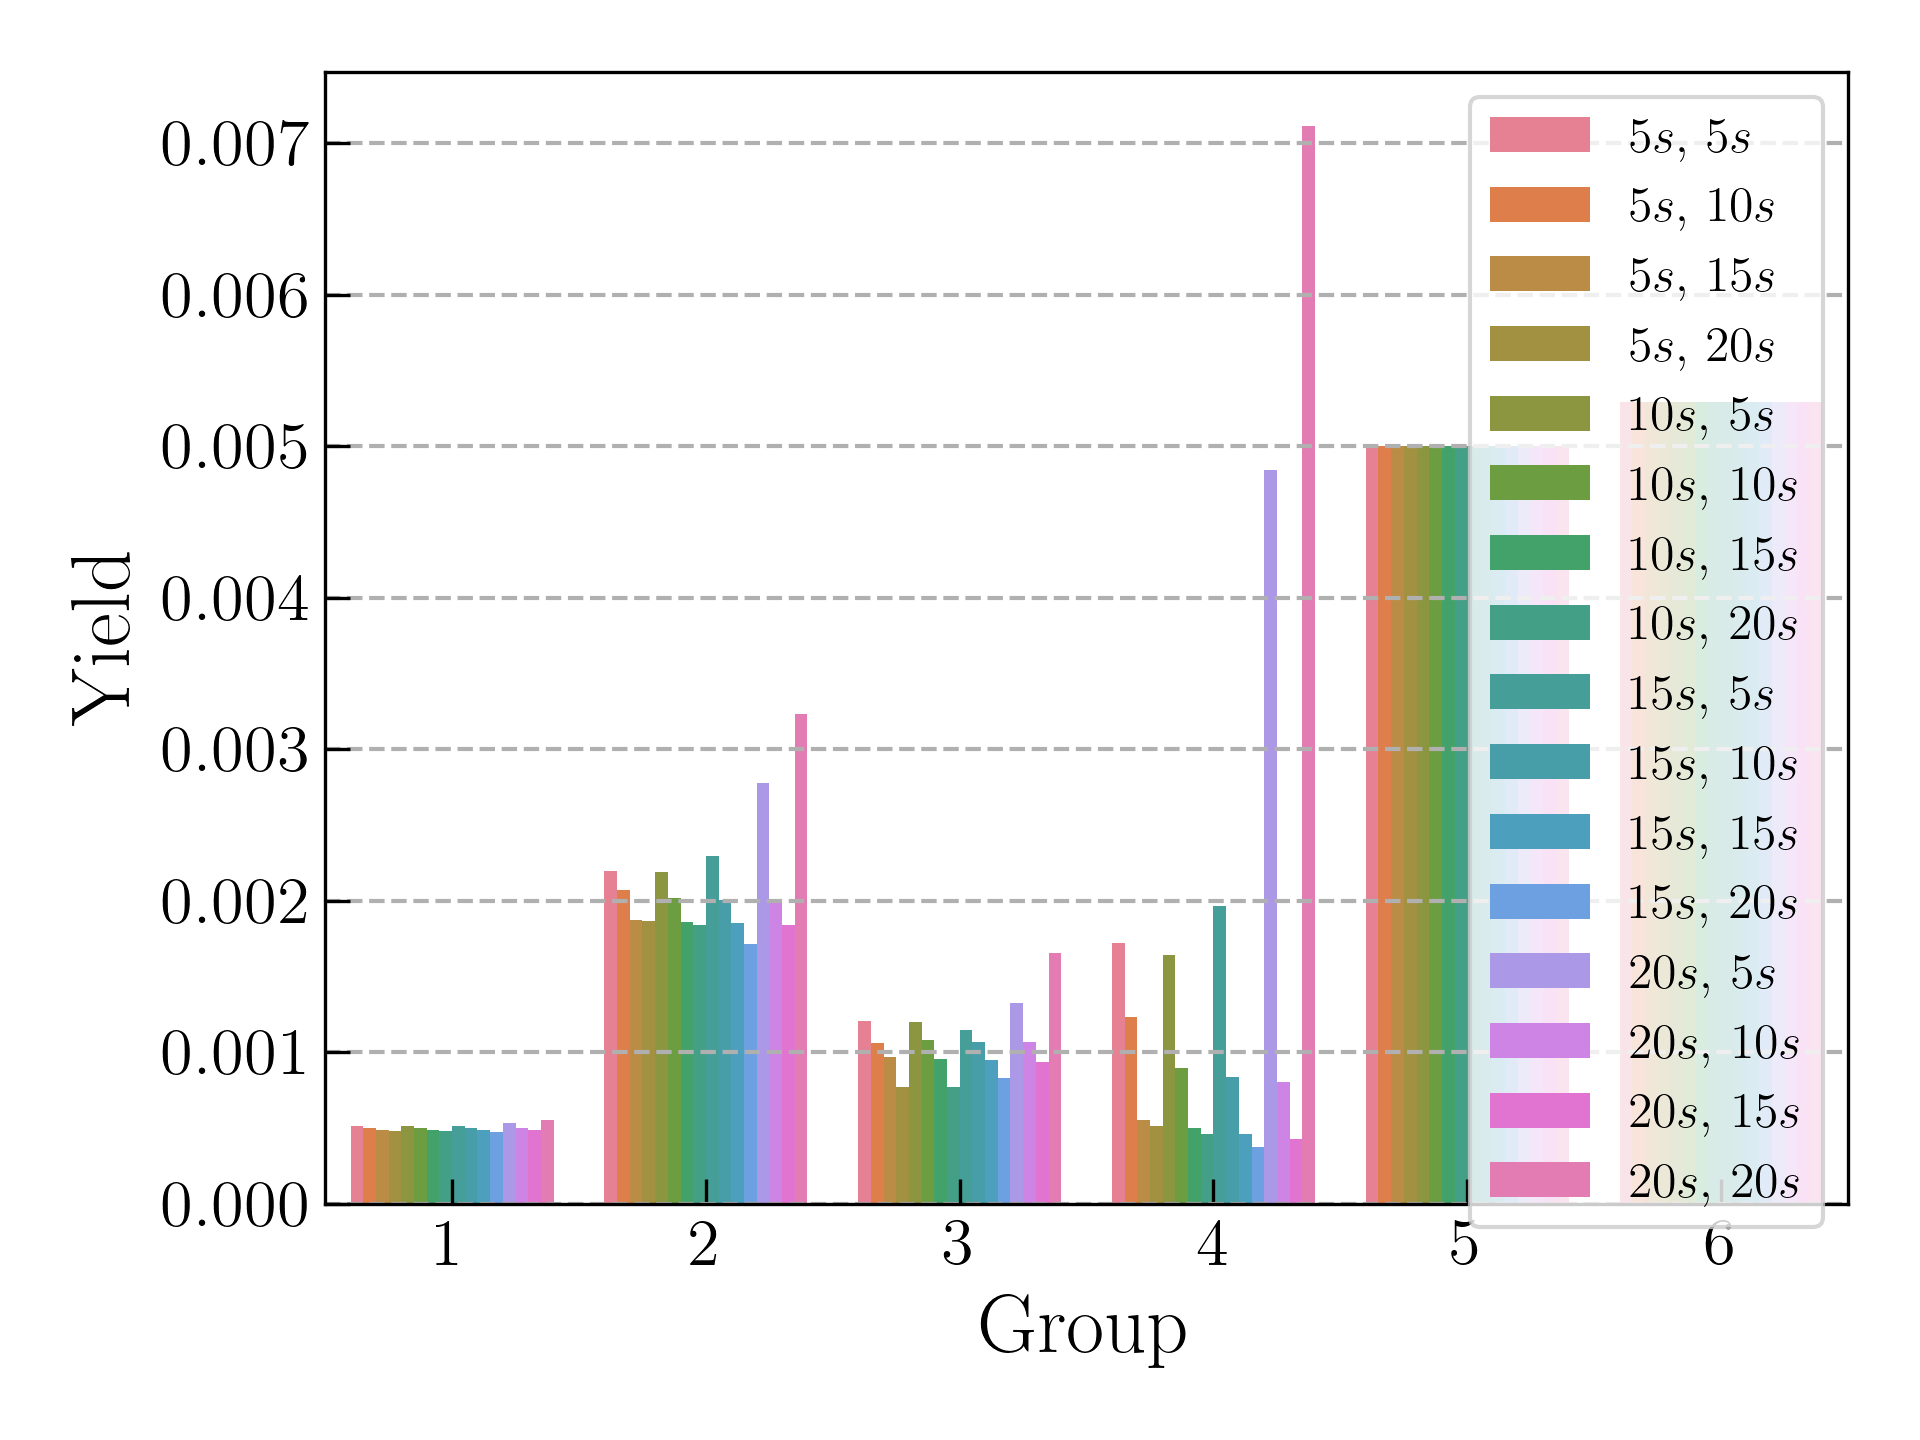
\includegraphics[width=\linewidth]{images/yields-csvs-restimestudy.png}
    \caption{Group yields for various residence times during irradiation in OpenMC.}
    \label{fig:yields-restimestudy}
\end{figure}

\begin{table}[H]
    \centering
    \begin{tabular}{llcc}
    \hline
$\tau_{in}$ $[s]$ & $\tau_{ex}$ $[s]$  & $\bar{\nu}_d$ & $\bar{T}$ $[s]$ \\
\hline
5$s$ & 5$s$ & 0.015940 & 8.101997\\
5$s$ & 10$s$ & 0.015165 & 8.030291 \\
5$s$ & 15$s$ & 0.014179 & 8.293764 \\
5$s$ & 20$s$ & 0.013929 & 7.770002 \\
10$s$ & 5$s$ & 0.015851 & 8.113214 \\
10$s$ & 10$s$ & 0.014790 & 8.234031 \\
10$s$ & 15$s$ & 0.014109 & 8.304067 \\
10$s$ & 20$s$ & 0.013845 & 7.819340 \\
15$s$ & 5$s$ & 0.016220 & 7.869896 \\
15$s$ & 10$s$ & 0.014718 & 8.240623 \\
15$s$ & 15$s$ & 0.014051 & 8.310107 \\
15$s$ & 20$s$ & 0.013693 & 8.191821 \\
20$s$ & 5$s$ & 0.019775 & 7.537696 \\
20$s$ & 10$s$ & 0.014672 & 8.244369 \\
20$s$ & 15$s$ & 0.013996 & 8.313858 \\
20$s$ & 20$s$ & 0.022849 & 7.536158 \\
\hline
    \end{tabular}
    \caption{Effect of residence times on the total delayed neutron yield and average half-life.}
    \label{tab:omc-restimestudy}
\end{table}

\subsubsection{Combined Removal Rates and Residence Times}